\chapter{Cadre de l'assurance vie et contexte réglementaire}
\label{chap:cadre_assurance_vie_et_contexte_reglementaire}

%%%%%%%%%%%%%%%%%%%%%%%%%%%%
% L'évolution récente des taux directeurs
%%%%%%%%%%%%%%%%%%%%%%%%%%%%



\section{L'évolution récente des taux directeurs}

Longtemps maintenus à des niveaux historiquement bas, les taux d'intérêt ont connu au cours des dernières années une volatilité sans précédent depuis la création de la zone euro : d'abord tirés vers le bas par des politiques monétaires très accommodantes destinées à soutenir l'économie, ils ont ensuite été relevés à une vitesse inédite pour juguler un retour de l'inflation, avant d'amorcer une nouvelle détente. Comprendre les mécanismes qui gouvernent cette évolution est indispensable pour saisir l'environnement dans lequel opère aujourd'hui l'assurance vie.

\subsection{Les banques centrales et leurs politiques monétaires}
\subsubsection{Qu'est-ce qu'un taux d'intérêt ?}
Un \textbf{taux d'intérêt} est le coût de l'emprunt d'argent. Un taux d'intérêt est généralement exprimé en pourcentage annuel. Il existe plusieurs types de taux d'intérêt ; les deux principaux sont le taux d'intérêt nominal et le taux d'intérêt réel. \cite{banque_de_france1}

\begin{itemize}
    \item Le \textbf{taux d'intérêt nominal} correspond au taux indiqué dans un quelconque contrat (prêt, obligation, etc.), et c'est celui qui est réellement acquitté.
    \item Le \textbf{taux d'intérêt réel} est le taux d'intérêt ajusté par l'inflation. Il représente le coût réel de l'emprunt et de l'épargne après avoir pris en compte la perte de pouvoir d'achat due à l'inflation. Le taux d'intérêt réel peut être calculé en soustrayant le taux d'inflation du taux d'intérêt nominal.
    \begin{equation}
        \text{Taux d'intérêt réel} = \text{Taux d'intérêt nominal} - \text{Taux d'inflation}
    \end{equation}
\end{itemize}

Les taux d'intérêt dépendent de nombreux facteurs, notamment des politiques monétaires des banques centrales, de la durée des emprunts, de la solvabilité des emprunteurs (risque de crédit) ainsi que de la nature des biens ou services financés. Les banques centrales jouent un rôle déterminant dans la fixation des taux à court terme, pour que les taux à long terme soient alignés à leurs objectifs. En outre, les taux à court terme sont généralement inférieurs aux taux à long terme en raison de la prime de risque associée à la durée plus longue de l'emprunt. \cite{banque_de_france1}

\subsubsection{Les banques et le marché interbancaire}
%%% Chercher le cours sur les banques

Une \textbf{banque} est une institution financière qui offre une gamme de services financiers, notamment la gestion des dépôts, l'octroi de prêts, la facilitation des paiements et la fourniture de services d'investissement. Les banques jouent un rôle crucial dans l'économie en facilitant les transactions financières, en fournissant du crédit aux entreprises et aux particuliers, et en contribuant à la stabilité financière. Elles agissent comme des intermédiaires entre les épargnants qui déposent de l'argent et les emprunteurs qui ont besoin de fonds pour financer leurs projets ou leurs dépenses. Les banques peuvent être classées en différentes catégories, telles que les banques commerciales, les banques d'investissement, les banques centrales et les banques coopératives, chacune ayant des fonctions spécifiques dans le système financier.

La banque la plus influente à l'échelle mondiale est la \textbf{Réserve fédérale américaine} ou \textit{Federal Reserve System}, souvent raccourcie en \textbf{Fed}. C'est la banque centrale des États-Unis. Elle a été créée en 1913 et elle est chargée de la politique monétaire du pays. La Fed est une entité indépendante du gouvernement, ce qui lui permet de prendre des décisions de politique monétaire sans être influencée par des considérations politiques à court terme.

De son côté, la \textbf{Banque centrale européenne (BCE)} est l'institution responsable de la politique monétaire de la zone euro. Elle fait partie, avec les banques centrales nationales des pays membres, d'un organe de l'Union européenne appelé \textbf{l'Eurosystème}.

La BCE a été créée en 1998 et elle est chargée de maintenir la stabilité des prix et de soutenir la croissance économique dans les pays qui utilisent l'euro comme monnaie. La BCE fixe les taux directeurs, qui influencent les taux d'intérêt à court terme dans la zone euro, et elle mobilise différents instruments de politique monétaire afin d'atteindre ses objectifs. \newline
L'objectif principal de la BCE est de maintenir l'inflation à un niveau proche et légèrement inférieur à 2\% ; niveau jugé suffisamment bas pour préserver le pouvoir d'achat tout en étant assez élevé pour garantir une flexibilité économique et une efficacité de la politique monétaire afin d'éviter les risques de déflation.

Les différents taux directeurs de la BCE sont les suivants \cite{banque_de_france_taux_directeurs} :

\begin{itemize}
    \item Le principal taux directeur est le \textbf{taux d'intérêt des opérations principales de refinancement}. C'est le taux auquel la BCE prête de l'argent aux banques commerciales pour une durée d'une semaine. 
    \item Le \textbf{taux d'intérêt de la facilité de prêt marginal} est le taux auquel les banques commerciales peuvent emprunter de l'argent auprès de la BCE en cas de besoin urgent de liquidités, pour une durée de 24 heures. Il est plus élevé que le taux de refinancement principal, ce qui incite les banques à éviter de recourir à cette facilité sauf en cas de nécessité absolue.
    \item Le \textbf{taux de la facilité de dépôt} est le taux auquel les banques commerciales peuvent déposer de l'argent auprès de la BCE pour une durée de 24 heures. 
\end{itemize}

Ainsi, les taux directeurs désignent les taux définis par la Banque centrale européenne pour piloter le coût de la monnaie au sein de l'économie. Lorsqu'une banque centrale augmente ses taux directeurs, la BCE augmente le coût auquel les banques peuvent obtenir des liquidités lors des opérations principales de refinancement. Comme le refinancement devient plus cher, les taux à court terme entre établissements augmentent également. Par transmission, les taux du marché monétaire et, plus largement, les taux appliqués aux ménages et aux entreprises tendent alors à augmenter. Des taux plus élevés réduisent alors la demande d'emprunt et peuvent aussi durcir les critères d'octroi. Enfin la création monétaire se modère et la demande globale est freinée, ce qui contribue à atténuer les pressions inflationnistes. À l'inverse, lorsque la banque centrale baisse ses taux directeurs, elle facilite l'accès des banques à la liquidité, ce qui tend à faire diminuer les taux auxquels elles se prêtent mutuellement. Le \textbf{marché interbancaire} est précisément le marché financier sur lequel les banques échangent des fonds à court terme afin de gérer leur trésorerie et leurs besoins de liquidité. Il s'agit d'un marché de gré à gré où les établissements bancaires empruntent et prêtent directement entre eux à des taux appelés taux interbancaires. Dans la zone euro, ce taux à 24 heures était le taux EONIA (Euro Overnight Indexed Average) et il a été remplacé, fin 2019, par le taux €STR (Euro Short-Term Rate). Ce taux interbancaire fluctuait entre un "taux plancher" (le taux de la facilité de dépôt) et un "taux plafond" (le taux de la facilité de prêt marginal). En effet, les banques n'ont pas d'intérêt à emprunter à un taux supérieur au taux de la facilité de prêt marginal, ni à prêter à un taux inférieur au taux de la facilité de dépôt. Ce système, appelé "corridor de taux", a été en vigueur jusqu'à la crise de 2008. À la suite de la crise, l'Eurosystème a mis en œuvre des mesures de politique monétaire non conventionnelles afin de soutenir la reprise économique, ce qui s'est traduit par une augmentation significative de la liquidité. Dans ce contexte d'abondance de liquidités, les banques ont moins eu recours au refinancement interbancaire, entraînant une baisse durable du taux interbancaire jusqu'au niveau du taux de la facilité de dépôt. Et ce dernier taux est devenu le principal taux directeur. Ainsi, en agissant sur ses taux directeurs, la Banque centrale européenne influence directement les conditions de financement sur le marché interbancaire et, plus largement, l'ensemble du financement de l'économie.


\subsection{Le contexte historique de l'influence des banques centrales}

Les banques centrales jouent donc un rôle majeur dans la détermination des conditions de financement et dans la gestion de l'inflation. La figure \ref{fig:tx_directeurs_bce} illustre l'évolution des taux directeurs de la BCE depuis 2000, en mettant en évidence les différentes phases de politique monétaire adoptées par l'institution au fil du temps. Nous pouvons ainsi observer trois pics de taux élevés qui correspondent à la bulle internet au début des années 2000, à la crise des subprimes en 2008, puis à la période récente du Covid-19 et des tensions géopolitiques. Nous observons aussi une longue période de taux bas qui correspond à une période marquée par les politiques monétaires accommodantes adoptées par la BCE pour soutenir la croissance économique face à une inflation trop faible. 


\begin{figure}[H]
    \centering
    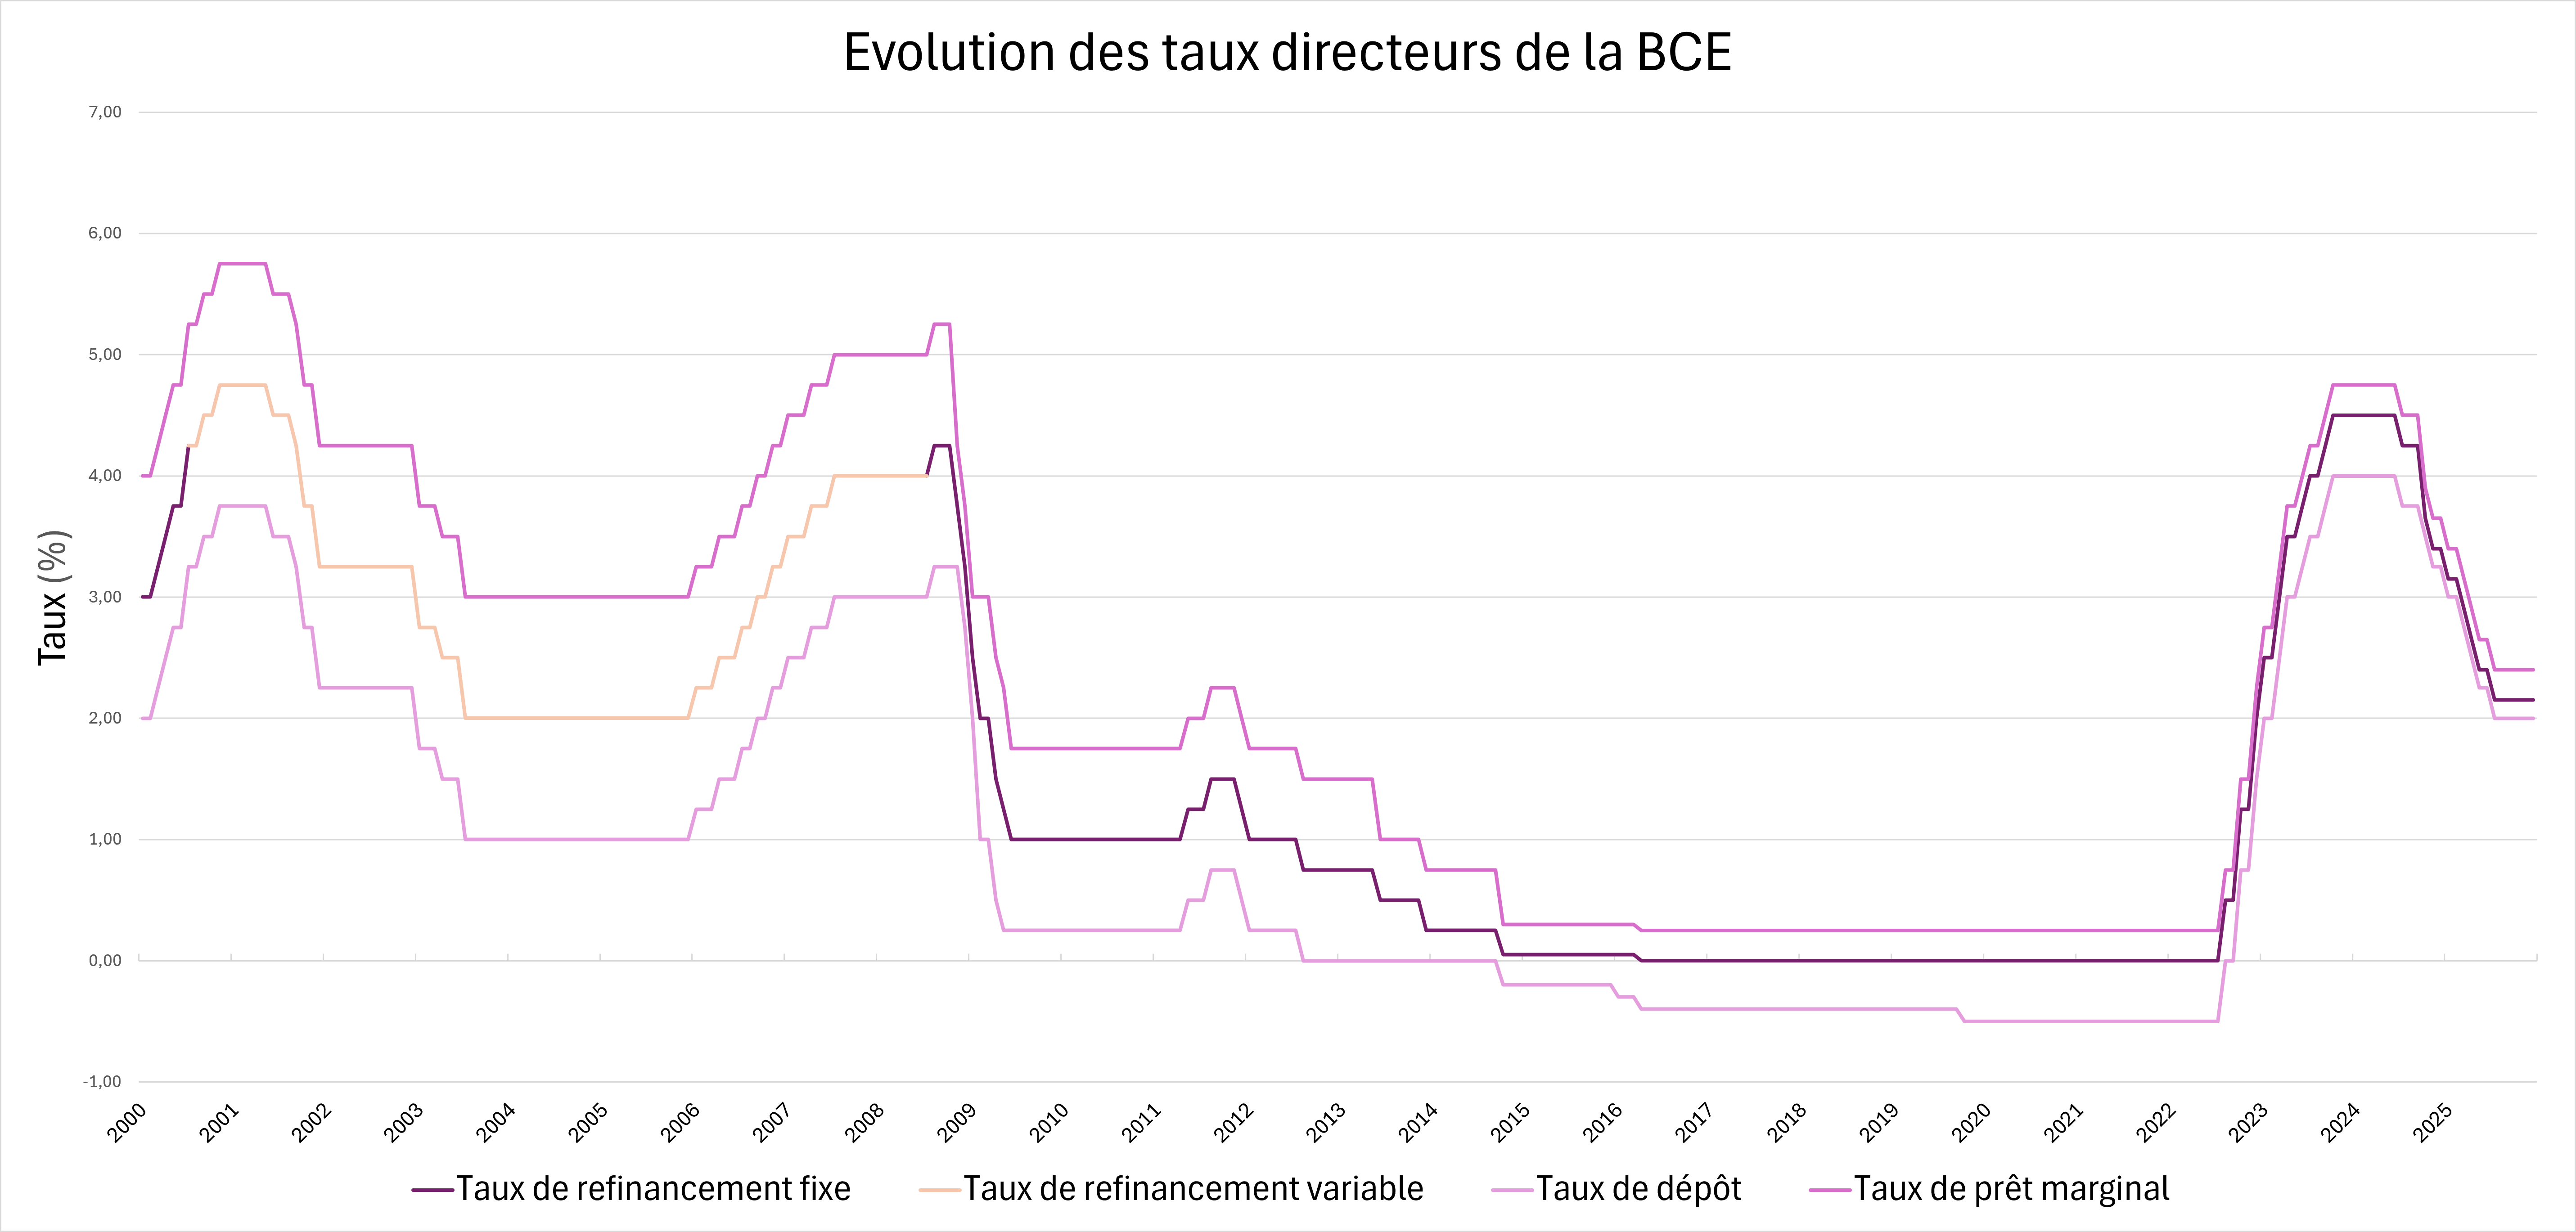
\includegraphics[scale=0.36]{images/evolution_tx_directeurs_bce.png}
    \caption{Evolution des taux directeurs de la BCE entre 2000 et 2025}
    \label{fig:tx_directeurs_bce}
\end{figure}

Entre juin 2000 et octobre 2008, les opérations principales de refinancement de l'Eurosystème étaient menées sous la forme d'appels d'offres à taux variable. Dans ce cadre, le taux retenu correspondait au taux minimal de soumission, c'est-à-dire au taux plancher en dessous duquel les établissements bancaires ne pouvaient pas présenter leurs offres. Toutefois, le 8 octobre 2008, dans le contexte de la crise financière, la BCE a annoncé qu'à compter de l'opération réglée le 15 octobre 2008, les opérations principales de refinancement hebdomadaires seraient désormais conduites selon une procédure à taux fixe.


Depuis la crise financière de 2008, la BCE a vu son rôle renforcé dans la gestion de la politique monétaire de la zone euro. Elle a joué un rôle central dans la stabilisation de l'économie européenne grâce à sa gestion active des taux d'intérêt. Nous pouvons recenser trois principales phases que nous allons détailler ci-dessous :

\subsubsection{L'environnement de taux nuls après la crise financière}

Dans un premier temps, après la crise financière de 2008, la situation économique s'est avérée particulièrement difficile, caractérisée par une forte récession et une inflation basse ; en 2009, le PIB réel de la zone euro s'est ainsi contracté de 4,0 \%, tandis que l'inflation annuelle moyenne est tombée à 0,3 \%. La BCE a donc adopté une politique monétaire accommodante en réduisant les taux d'intérêt de manière significative. En effet la BCE a abaissé le taux de refinancement de 4 à 1\% en 2009, puis à 0,75\% en juillet 2012, et enfin jusqu'à 0,05\% en 2014. Cette politique soutient la croissance par le mécanisme de transmission monétaire. Lorsque la BCE abaisse ses taux directeurs, elle réduit d'abord le coût auquel les banques se refinancent auprès de l'Eurosystème et influence à la baisse l'ensemble des taux du marché monétaire et, progressivement, les taux appliqués aux ménages et aux entreprises. Le crédit devient alors moins coûteux : les ménages peuvent davantage financer leurs achats immobiliers ou de consommation, tandis que les entreprises peuvent investir à un coût plus faible. Cette détente des conditions de financement stimule donc la demande, c'est-à-dire la consommation et l'investissement, ce qui soutient l'activité économique. En outre, dans un contexte d'inflation trop faible, une politique accommodante vise aussi à éviter que ménages et entreprises ne reportent leurs dépenses dans l'attente de prix plus bas, ce qui aggraverait encore le ralentissement économique. Cependant, malgré ces mesures, l'économie européenne est restée fragile pendant plusieurs années, ce qui a conduit la BCE à adopter des mesures supplémentaires pour stimuler l'économie.

À partir de 2015, la BCE met en place un programme de Quantitative Easing en complément de sa politique de taux d'intérêt bas. C'est l'\textit{Asset Purchase Program }(APP).
Le \textbf{quantitative easing (QE)} \cite{banque_de_france3} ou assouplissement quantitatif est une politique monétaire non conventionnelle utilisée par les banques centrales. Cette politique est généralement mise en œuvre pour lutter contre le risque de déflation et pour relancer l'économie lorsque les taux d'intérêt sont déjà très bas. Le QE consiste, pour la banque centrale, à acheter massivement des actifs financiers auprès des banques commerciales et d'autres institutions financières. Les actifs achetés sont le plus souvent des obligations d'État, mais ils peuvent aussi inclure des titres de dette privée.
Ainsi, le programme APP permet d'injecter des liquidités dans l'économie et de soutenir la croissance économique dans la zone euro. À compter de mars 2015, ces achats représentent 60 milliards d'euros par mois, pour un montant initial supérieur à 1 100 milliards d'euros sur la période allant jusqu'à septembre 2016. Ce volume est ensuite progressivement étendu au fil du temps, si bien qu'à la fin de l'année 2022, l'Eurosystème détient 3 254 milliards d'euros d'encours au titre de l'APP.

Le mécanisme fonctionne de la manière suivante : en achetant ces titres, la BCE paie les vendeurs, principalement des banques commerciales, en créant de la monnaie centrale. Ces établissements voient ainsi leurs réserves augmenter, ce qui leur permet d'accorder davantage de crédits à l'économie réelle. Par ailleurs, ces achats massifs font augmenter la demande pour les obligations ainsi acquises. Or, le prix d'une obligation et son rendement évoluent en sens inverse : lorsque la demande pousse les prix à la hausse, les rendements baissent mécaniquement. Des taux plus bas signifient un crédit moins cher pour les ménages et les entreprises, ce qui encourage l'emprunt et l'investissement. Enfin, la création monétaire induite par ces achats contribue à relever l'inflation vers la cible de 2\,\%, en écartant le risque de déflation que craignait alors la BCE.

Finalement, l'APP agit simultanément sur la liquidité bancaire, les conditions de financement et les anticipations d'inflation, participant ainsi à la relance de l'activité économique dans la zone euro.

\subsubsection{La succession des chocs récents : pandémie, guerre en Ukraine et retour de l'inflation}

% mettre un graphique de l'évolution de l'inflation en Europe, il est déjà prêt. a voir pour mettre aussi la courbe de la France. peut etre changer le graphique pour y mettre explicitement l'IPC.
% chercher les infos/données sur le site de l'INSEE

Afin de préserver la transmission de la politique monétaire dans le contexte de la crise sanitaire, la BCE a réactivé des mesures non conventionnelles de soutien à l'économie. Elle a ainsi lancé, en mars 2020, le programme d'achats d'urgence face à la pandémie (\textit{Pandemic Emergency Purchase Program}, PEPP), destiné à limiter les tensions financières et à soutenir des économies fortement affectées par la pandémie. Ce dispositif est venu s'ajouter à l'APP, les actifs éligibles dans le cadre de ce dernier étant également éligibles au titre du PEPP. En 2022, l'encours d'actifs détenus par l'Eurosystème au titre de ce programme atteignait environ 1 700 milliards d'euros.

\begin{figure}[H]
    \centering
    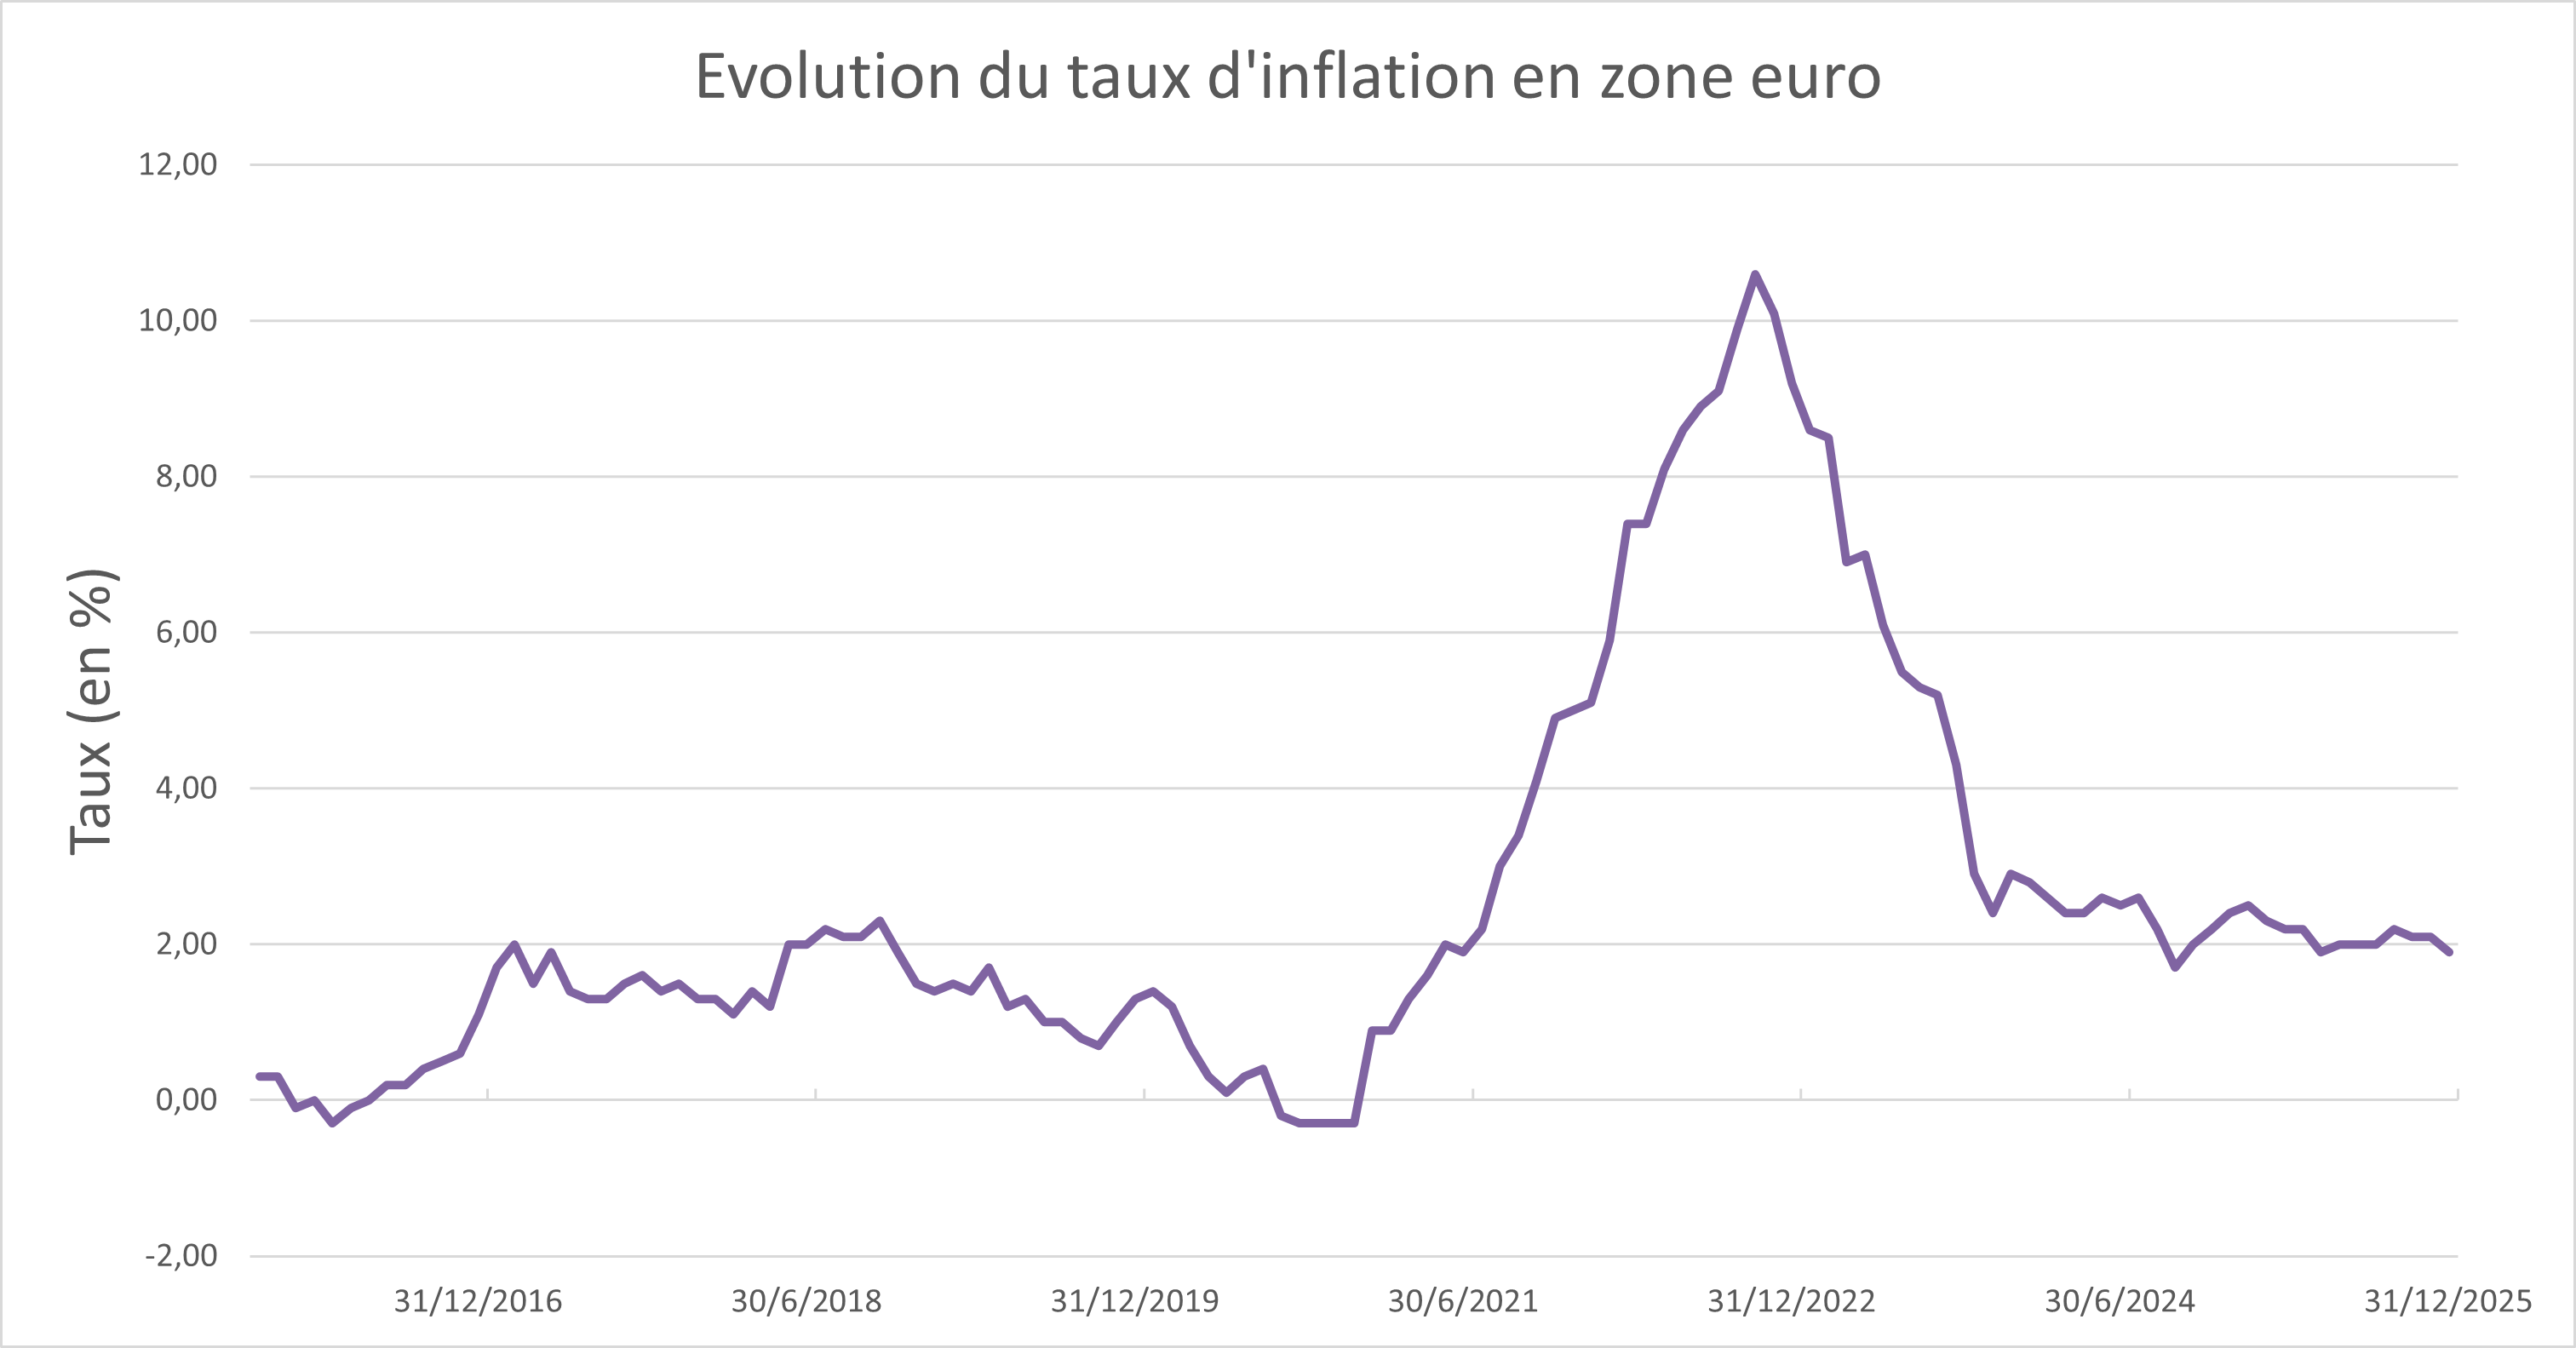
\includegraphics[scale=0.5]{images/tx_inflation_2016_2025.png}
    \caption{Evolution du taux d'inflation en Europe entre 2016 et 2025}
    \label{fig:tx_inflation}
\end{figure}

Toutefois, la sortie progressive de la crise sanitaire, marquée par la levée des confinements et la reprise de l'activité, a entraîné un fort rebond de la demande. Ce mouvement a alimenté les tensions inflationnistes comme le montre le pic d'inflation en 2022 (Figure \ref{fig:tx_inflation}). Celles-ci ont ensuite été accentuées par la guerre en Ukraine, notamment à travers la hausse des prix de l'énergie et des matières premières. Dans ce nouveau contexte, la BCE a dû infléchir sa stratégie monétaire et mettre fin à l'orientation très accommodante qui prévalait jusque-là. Elle a ainsi abandonné progressivement les politiques d'achats massifs d'actifs et est revenue à des instruments plus conventionnels. Ce changement de cap s'est matérialisé par une première hausse des taux directeurs en juillet 2022, suivie de plusieurs relèvements destinés à freiner l'inflation et à restaurer la stabilité macroéconomique dans la zone euro. Le taux de refinancement principal a ainsi été porté à 4,25 \% en septembre 2023. L'objectif de se resserrement monétaire était de durcir les conditions de financement afin de freiner la demande et d'éviter un ancrage durable de l'inflation à un niveau trop élevé. La hausse des taux a toutefois été interrompue à partir de septembre 2023, la BCE considérant alors que le niveau atteint était suffisamment restrictif et qu'il convenait de laisser se diffuser les effets, nécessairement retardés, du resserrement monétaire. Cette phase de taux élevés a entraîné un renchérissement du crédit, un ralentissement de l'investissement et de la demande, ainsi qu'un tassement du marché immobilier, mais elle a également contribué à la désinflation observée à partir de la fin de l'année 2023.

\subsubsection{La baisse des taux et sa stabilisation à 2\% en Europe}

Après avoir maintenu ses taux à un niveau élevé pendant plusieurs mois, la BCE a amorcé un cycle d'assouplissement lorsque le processus de désinflation est apparu suffisamment avancé. Le premier geste d'allègement est intervenu en juin 2024, après neuf mois de statu quo, l'institution estimant alors que le degré de restriction monétaire pouvait être atténué. Les ajustements ont ensuite été graduels, par paliers de 25 points de base : en octobre et décembre 2024, puis en janvier, mars, avril et juin 2025. À l'issue de cette baisse, le taux de la facilité de dépôt a été ramené à 2,00 \% et celui des opérations principales de refinancement à 2,15 \%.

Cet assouplissement s'est justifié par le recul de l'inflation. Il ne s'agissait plus de freiner brutalement l'activité, mais d'éviter de maintenir trop longtemps des conditions monétaires excessivement contraignantes alors que la dynamique des prix se rapprochait de la cible. Une fois le taux de dépôt revenu à 2,00 \%, la banque centrale a néanmoins suspendu ses ajustements, afin de laisser les effets des décisions passées se diffuser dans l'économie. En février puis en mars 2026, la BCE a ainsi maintenu ses paramètres inchangés, réaffirmant sa volonté d'ancrer durablement l'inflation à 2 \% à moyen terme, tout en tenant compte d'un environnement devenu plus incertain, notamment en raison des risques énergétiques et géopolitiques.

Les répercussions d'une telle détente monétaire sont globalement inverses de celles observées durant la phase de resserrement, mais leur transmission s'opère avec décalage. En principe, l'allègement progressif du coût du crédit qui en découle soutient l'investissement des entreprises, la consommation des ménages et, plus largement, la croissance. L'institution souligne d'ailleurs que les mesures d'assouplissement passées commencent à produire leurs effets. Toutefois, ce mécanisme n'est pas immédiat : le taux moyen appliqué aux encours de prêts immobiliers peut encore continuer à s'élever pendant un certain temps, en raison des effets retardés de l'ancien cycle restrictif. Par ailleurs, un environnement de taux plus bas tend à comprimer la rémunération de l'épargne sans risque, même s'il améliore parallèlement les conditions d'emprunt.

% inclure un graphique de la croissance du PIB en Europe, et mettre aussi la courbe de la France si possible. utile ? relation PIB - inflation ?



%%%%%%%%%%%%%%%%%%%%%%%%%%%%%
% L'assurance vie
%%%%%%%%%%%%%%%%%%%%%%%%%%%%%
\section{L'assurance vie}

\subsection{Les spécificités de l'assurance vie}

L'évolution des taux directeurs et, plus largement, de l'environnement monétaire constitue un élément central pour comprendre les transformations récentes du secteur financier. En effet, les choix de politique monétaire influencent directement les conditions de financement et le niveau des taux sans risque, qui jouent un rôle déterminant dans la valorisation des engagements de long terme. Dans ce contexte, il convient désormais d'examiner plus spécifiquement le cas de l'assurance vie, dont le modèle économique est particulièrement sensible aux variations de taux d'intérêt.

\textbf{L'assurance vie} est un contrat d'assurance dans lequel un souscripteur verse des primes à un assureur, qui s'engage en contrepartie à verser un capital ou une rente à un bénéficiaire déterminé. Ce produit a pour objectif principal de constituer et de valoriser une épargne sur le long terme en générant des intérêts. Le bénéficiaire peut être l'assuré lui-même lorsqu'il procède au rachat de son contrat de son vivant ou au terme d'un contrat à durée limitée. Le bénéficiaire peut aussi être une personne désignée à l'avance en cas de décès de l'assuré. L'assurance vie constitue ainsi à la fois un support d'épargne et un outil de transmission patrimoniale, bénéficiant d'un cadre juridique et fiscal spécifique.
Ce contrat est aussi un outil de prévoyance, puisqu'il offre la possibilité de protéger ses proches en leur garantissant le versement d'une somme d'argent en cas de décès. 

La durée du contrat conclu par le souscripteur dépend de la vie de l'assuré. Il existe trois catégories de contrats : le contrat en cas de vie, le contrat en cas de décès et le contrat mixte.

\begin{itemize}
    \item Le \textbf{contrat en cas de vie} permet de constituer une épargne. Il prévoit que le capital ou la rente sera versé à l'assuré à une date déterminée, à condition que celui-ci soit encore en vie à cette échéance. Ce type de contrat est souvent utilisé pour financer un projet futur ou anticiper la retraite.
    \item Le \textbf{contrat en cas de décès} permet de protéger les proches de l'assuré en cas de décès. Ainsi, le versement par l'assureur est déclenché par le décès de l'assuré, et le capital ou la rente est versé au bénéficiaire désigné. 
    \item Le \textbf{contrat mixte}, aussi appelé contrat en cas de vie et de décès, combine les caractéristiques des deux contrats précédents. Il permet à la fois de constituer une épargne et d'assurer une protection financière pour les bénéficiaires de l'assuré en cas de décès.
\end{itemize}

En assurance vie, le souscripteur peut choisir entre deux catégories de contrats.  D'une part, les contrats dits « monosupports » sont exclusivement investis en fonds en euros. D'autre part, les contrats « multisupports », aujourd'hui majoritaires sur le marché, permettent de répartir l'épargne entre un fonds en euros et différents supports en unités de compte.
Parmi les différents supports que peut comporter un contrat d'assurance vie, on distingue le fonds en euros, les unités de compte (UC) et le contrat eurocroissance. Ces trois formes de contrats se différencient essentiellement par la nature actifs sous-jacents, le niveau de risque supporté par le souscripteur et les perspectives de rendement offertes.

Le fonds en euros est la forme la plus sécurisée de l'assurance vie. Les sommes versées par le souscripteur sont investies uniquement sur des supports peu risqués, tels que des obligations d'État ou d'entreprises. Ce type de contrat présente un avantage majeur : le capital versé est entièrement garanti par l'assureur et il est possible de le retirer. Cela signifie que l'épargnant ne peut pas perdre les sommes investies, hors frais éventuels. En outre, les intérêts générés chaque année sont définitivement acquis grâce au mécanisme dit de « l'effet cliquet ». Ainsi, même si les performances futures diminuent, les gains déjà crédités demeurent acquis. Le contrat en euros convient donc particulièrement aux épargnants recherchant la sécurité et la stabilité, même si, en contrepartie, son rendement est généralement plus modéré.

Le contrat en unités de compte, à l'inverse, repose sur une logique de diversification et de recherche de performance. Les primes versées sont investies sur différents supports financiers, appelés unités de compte, qui peuvent être composés d'actions, d'obligations, de parts d'OPCVM (Organismes de Placement Collectif en Valeurs Mobilières), de SCPI (Sociétés de Placement Immobilier) ou encore d'autres instruments financiers. Contrairement au fonds en euros, le capital investi n'est pas garanti : seule la quantité d'unités de compte détenues l'est. La valeur du contrat varie ainsi à la hausse comme à la baisse selon l'évolution des supports d'investissement choisis. Le souscripteur est donc exposé à un risque de perte en capital, en contrepartie d'une espérance de rendement potentiellement plus élevée à long terme. Ce type de contrat s'adresse principalement aux épargnants disposés à accepter une part de risque afin de bénéficier de perspectives de valorisation plus importantes.

À mi-chemin entre le fonds en euros et les unités de compte, le contrat eurocroissance constitue une formule intermédiaire entre sécurité et recherche de rendement. Il vise à offrir une espérance de performance supérieure à celle du fonds en euros classique, tout en prévoyant une garantie du capital uniquement à l'échéance du contrat, fixée à un minimum de huit ans. En cas de rachat avant ce terme, cette garantie ne s'applique pas. Pendant la durée du contrat, l'épargne évolue au fil du temps selon les supports dans lesquels elle est investie. Dans cette logique, la gestion de l'épargne repose généralement sur une part initialement plus importante de supports dynamiques, puis sur une sécurisation progressive à mesure que l'échéance approche. Le contrat eurocroissance cherche ainsi à concilier un potentiel de rendement plus élevé qu'un fonds en euros avec une garantie en capital à long terme.

Ces trois types de contrats répondent ainsi à des objectifs patrimoniaux différents. Le contrat en euros privilégie la sécurité du capital, le contrat en unités de compte favorise la recherche de rendement, tandis que le contrat eurocroissance constitue une solution intermédiaire, adaptée aux épargnants disposés à immobiliser leur épargne pendant plusieurs années afin de bénéficier d'un compromis entre garantie et performance. Le choix entre ces supports dépend donc du profil de l'investisseur, de son horizon de placement et de sa tolérance au risque.


\subsubsection{L'assurance vie en France : poids économique et dynamiques récentes}

L'assurance vie occupe une place centrale dans l'épargne financière des ménages français. Elle constitue à la fois un produit d'épargne de long terme, un outil de transmission patrimoniale et une source de financement importante pour l'économie. Par l'ampleur des encours qu'elle représente, elle figure parmi les principaux placements détenus par les ménages (Figure \ref{fig:encours_menages_francais_T42025}), ce qui en fait un secteur stratégique aussi bien pour les assureurs que pour les pouvoirs publics.

\begin{figure}[H]
    \centering
    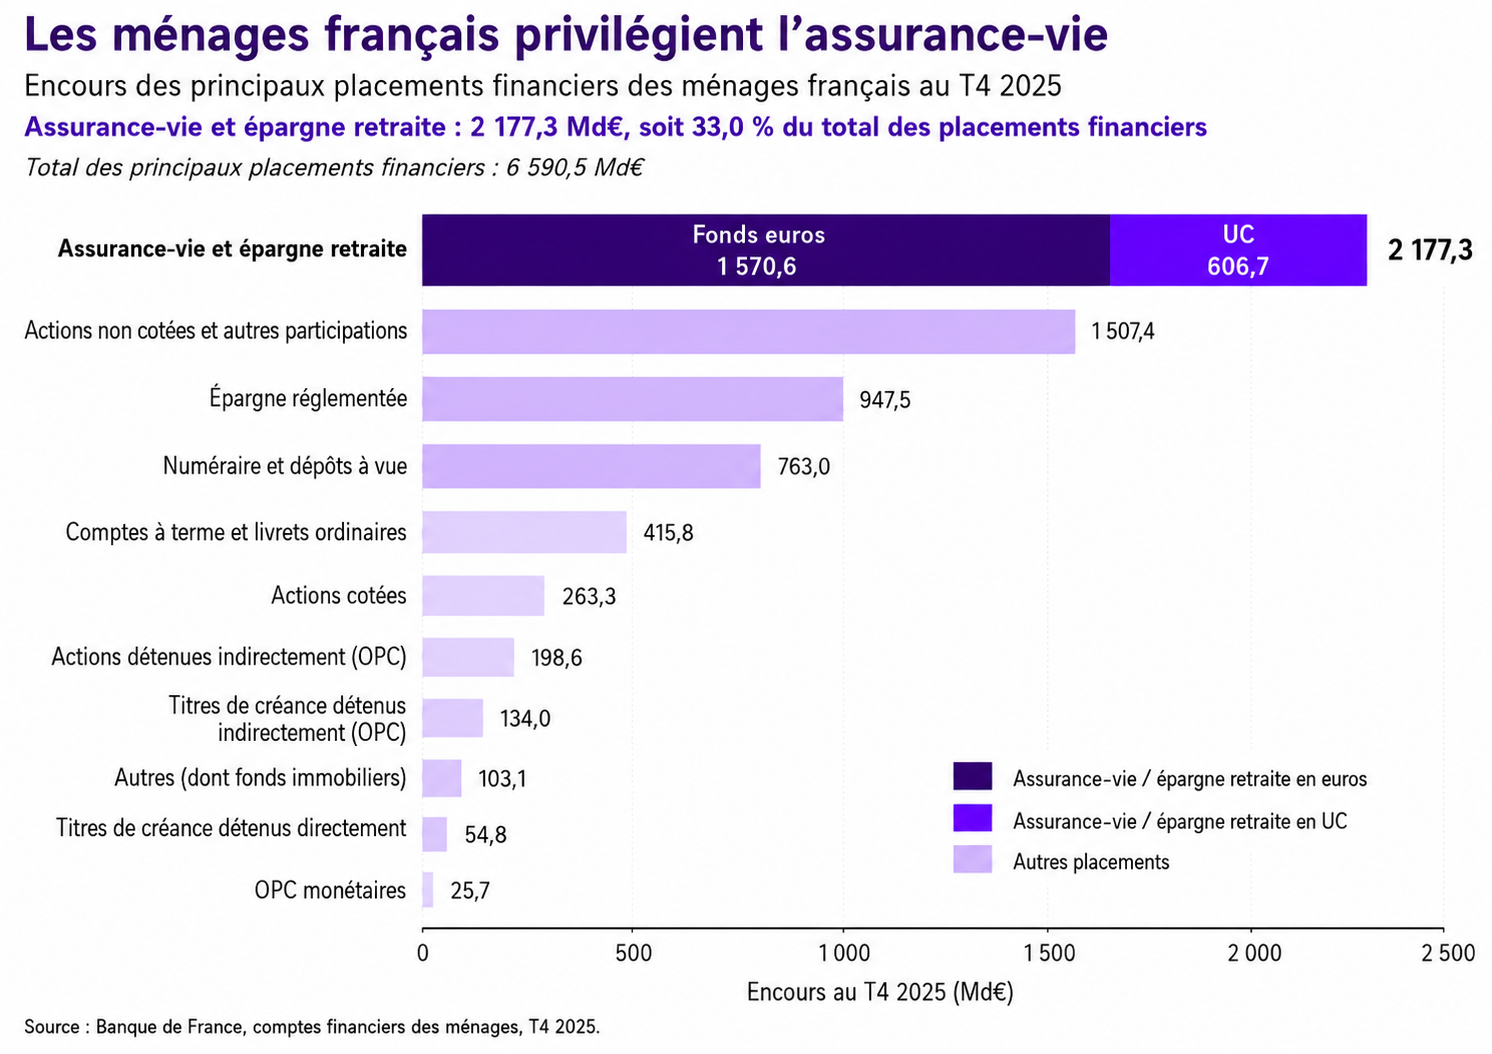
\includegraphics[scale=0.25]{images/encours_menages_francais_T42025.png}
    \caption{Encours d'épargne financière des ménages français à la fin de 2025}
    \label{fig:encours_menages_francais_T42025}
\end{figure}


Les principaux chiffres du marché à la fin de l'année 2025 sont présentés dans le tableau \ref{tab:chiffres_cles_assurance_vie_france}. L'encours total de l'assurance vie en France s'élève à 2\,107,0 Md€, contre 1\,985,8 Md€ un an plus tôt, soit une progression de 6,1 \%. Sur la même période, les cotisations atteignent 192,1 Md€, tandis que les prestations s'établissent à 141,4 Md€, conduisant à une collecte nette de 50,6 Md€. Ces résultats traduisent un regain de dynamisme du marché, dans un contexte marqué par l'évolution de l'environnement financier et par une réorientation progressive des comportements d'épargne.

\begin{table}[h]
    \centering
    \renewcommand{\arraystretch}{1.15}
    \begin{tabular}{lcccc}
        \toprule
        \textbf{Indicateurs (Md€)} & \textbf{Fonds en euros} & \textbf{Unités de compte} & \textbf{Ensemble} & \textbf{Var. / 2024} \\
        \midrule
        Cotisations    & 117,0   & 75,1  & 192,1   & +9,8 \% \\
        Prestations    & 108,9   & 32,6  & 141,4   & -3,4 \% \\
        Collecte nette & 8,1     & 42,5  & 50,6    & +22,1 Md€ \\
        \midrule
        Encours        & 1 432,8 & 674,2 & 2 107,0 & +6,1 \% \\
        \bottomrule
    \end{tabular}
    \caption{Chiffres clés de l'assurance vie en France à la fin de 2025}
    \label{tab:chiffres_cles_assurance_vie_france}
\end{table}

Le tableau \ref{tab:chiffres_cles_assurance_vie_france} met également en évidence la structure du marché. Les fonds en euros demeurent majoritaires dans les encours, avec 1\,432,8 Md€, soit environ 68 \% du total, contre 674,2 Md€ pour les unités de compte, qui représentent près de 32 \%. Cette répartition confirme que la sécurité du capital reste un critère déterminant pour une large part des épargnants. Toutefois, l'analyse des flux montre une dynamique différente : les unités de compte représentent près de 39 \% des cotisations de l'année et plus de 84 \% de la collecte nette. Elles contribuent donc très fortement à la croissance récente du marché.

Ces évolutions traduisent une transformation progressive de l'assurance vie en France. D'un côté, les fonds en euros conservent une place centrale en raison de la garantie en capital qu'ils offrent et de leur rôle de support sécuritaire au sein des contrats. De l'autre, les unités de compte occupent une place croissante dans les flux, sous l'effet de la recherche de rendement, de la diversification des allocations et des orientations commerciales et réglementaires observées ces dernières années. Le marché de l'assurance vie repose ainsi sur un équilibre entre sécurité et performance.

Enfin, ces données mettent en évidence un point essentiel pour l'analyse du secteur : l'assurance vie est directement sensible à l'environnement de taux d'intérêt. Les variations de taux influencent en effet le rendement servi sur les fonds en euros, l'attractivité relative des différents supports, les arbitrages des souscripteurs ainsi que les conditions de gestion actif-passif des assureurs. Dès lors, l'étude des chiffres du marché français ne constitue pas seulement un état des lieux quantitatif ; elle permet également de mieux comprendre pourquoi l'incertitude entourant les taux directeurs représente aujourd'hui un enjeu majeur pour l'assurance vie.

%%%%%%%%%%%%%%%%%%%%%%%%%%%%%
% L'impact théorique des taux sur l'assurance vie
%%%%%%%%%%%%%%%%%%%%%%%%%%%%%
\section{L'impact stratégique des taux sur l'assurance vie pour les assureurs}

Dans les parties précédentes, il a été mis en évidence que les taux directeurs ont connu des évolutions marquées au cours des dernières années, sous l'effet notamment des orientations de politique monétaire adoptées par les banques centrales. Nous avons également vu que l'assurance vie est un produit d'épargne à long terme qui repose de façon importante sur les obligations. Dans ce contexte, la maîtrise du risque de taux représente un enjeu stratégique majeur pour les assureurs, dans la mesure où l'environnement de taux influence simultanément leur rentabilité, ainsi que la compétitivité de leurs offres en assurance vie.

\subsection{L'effet d'un environnement de taux bas}

L'EIOPA souligne que la période prolongée de taux bas a exercé une pression significative sur les assureurs, en affectant leur allocation d'actifs, en accentuant le risque de réinvestissement et en pesant sur leur rentabilité comme sur leur solvabilité, en particulier pour les assureurs vie proposant des garanties élevées. Ce contexte de taux bas a été l'enjeu majeur des années 2010 pour les assureurs vie.

Le premier effet du contexte de taux bas a touché le cœur même du modèle économique des fonds en euros. Historiquement, ces supports reposent sur une double promesse : d'une part, la garantie en capital et, d'autre part, l'attribution d'un rendement annuel, alimenté principalement par les revenus issus du portefeuille obligataire détenu par l'assureur. Or, à la suite de la crise financière de 2008, la baisse durable des taux souverains et obligataires a fait diminuer cette source de rémunération. Les nouvelles obligations achetées par les assureurs généraient en effet des coupons de plus en plus faibles, ce qui a conduit à une compression progressive de la marge financière dégagée sur les fonds en euros. 

L'ajustement à la baisse des rendements n'a toutefois pas été immédiat, en raison de l'inertie propre au portefeuille d'actifs des assureurs. En assurance vie, le portefeuille obligataire se renouvelle progressivement : une part importante des titres acquis dans un environnement de taux plus élevés continue, pendant plusieurs années, à verser des coupons supérieurs aux taux de marché et, lorsque les taux baissent, ces obligations anciennes se retrouvent en outre en situation de plus-values latentes. Il existe ainsi une véritable latence dans la transmission des variations de taux à la rémunération effective des actifs : la baisse des taux de marché n'affecte pas instantanément le rendement moyen du portefeuille, mais elle finit par s'imposer au fur et à mesure que les obligations anciennes arrivent à échéance, sont remboursées ou cédées, puis remplacées par des titres offrant des coupons plus faibles. À mesure que ce renouvellement s'opère, la marge financière se comprime, ce qui exerce une pression croissante sur les rendements servis aux assurés, en particulier lorsque certains contrats comportent encore des garanties minimales élevées. Le taux minimum garanti (TMG), garanti pour une durée maximale de deux ans, correspond en effet au taux technique complété d'une fraction de la participation aux bénéfices dans les limites fixées par la réglementation ; lorsque les taux de marché restent durablement faibles, ces engagements deviennent mécaniquement plus coûteux à financer. Cette configuration, particulièrement marquée entre 2015 et 2022, a donc placé les assureurs dans une situation de tension progressive entre, d'un côté, des actifs dont le rendement se dégradait avec retard mais continûment, et, de l'autre, des engagements de rendement hérités d'un environnement de taux plus favorable.

\subsubsection{L'impact sur le passif}

Face à la compression progressive de leur marge financière, les assureurs ont d'abord cherché à ajuster le passif, en réduisant les garanties proposées sur les affaires nouvelles et en limitant les taux servis. Cette évolution est encadrée et analysée par l'Autorité de contrôle prudentiel et de résolution (ACPR), qui constitue en France l'autorité de supervision prudentielle des établissements bancaires et des organismes d'assurance. Selon l'ACPR, au 1\textsuperscript{er} janvier 2016, le taux technique maximal applicable aux nouveaux contrats était plafonné à 0,5 \%, tandis que les pratiques de marché conduisaient le plus souvent à retenir un taux nul. Ce mouvement illustre une inflexion du modèle des fonds en euros : il ne s'agit plus de garantir contractuellement un rendement significatif, mais de conserver une souplesse suffisante dans la fixation future de la rémunération servie. Dans ce contexte, la baisse des garanties contractuelles a constitué un instrument central d'adaptation à la persistance d'un environnement de taux bas.

\subsubsection{L'utilisation de la Provision pour Participation aux Bénéfices (PPB)}

La deuxième réponse des assureurs a consisté à renforcer les mécanismes de lissage, au premier rang desquels figure la provision pour participation aux bénéfices (PPB). Concrètement, sur les contrats en euros, les assureurs doivent redistribuer aux assurés une part minimale de leurs résultats, correspondant schématiquement à 85 \% du résultat financier et à 90 \% du résultat technique ; cette participation aux résultats comprend les intérêts techniques, servis immédiatement au titre des garanties contractuelles, et la participation aux bénéfices, dont une partie peut être mise en réserve dans la PPB. La PPB constitue ainsi une réserve collective adossée aux contrats : elle permet de ne pas distribuer immédiatement l'intégralité de la participation aux bénéfices et d'en étaler la restitution dans le temps afin de lisser les rendements servis d'une année sur l'autre. En droit commun, les sommes qui y sont affectées doivent être reversées aux assurés ou réaffectées aux provisions mathématiques dans un délai maximal de huit ans.

Dans l'environnement de taux bas des années 2010, cet instrument est devenu central dans le pilotage des fonds en euros. En effet, les assureurs disposent d'une large flexibilité pour moduler la distribution de la participation aux bénéfices. Ainsi, afin de pallier une période de taux bas prolongée, ils ont doté massivement la PPB grâce aux titres à coupons élevés acquis dans les années précédentes. La dotation nette à la PPB est ainsi passée de 2,4 milliards d'euros en 2009 à 5,2 milliards en 2014, tandis que l'encours de PPB atteignait près de 29,0 milliards d'euros fin 2014. Le mouvement s'est poursuivi par la suite. En 2019, alors que le taux moyen de revalorisation des fonds euros des contrats individuels est tombé à 1,46 \% contre 1,83 \% en 2018. Cette baisse, plus marquée que celle du rendement de l'actif, a précisément permis aux assureurs de continuer à doter la PPB ; le niveau de provisionnement a ainsi atteint 4,7 \% des provisions d'assurance-vie, contre 4,3 \% en 2018 et 4,0 \% en 2017. Cette logique de lissage reste toutefois un amortisseur, et non une réponse structurelle au risque de taux. La Banque de France indiquait déjà en 2019 que la montée de la PPB permettait de réduire temporairement l'écart de rémunération entre les fonds en euros et les autres placements en cas de remontée des taux, mais qu'elle ne protégeait pas durablement les assureurs contre un scénario de hausse abrupte des taux à moyen terme.

\subsubsection{La réorientation de la collecte}

Le troisième axe stratégique a été commercial et a probablement constitué l'évolution la plus visible pour les épargnants : la réorientation progressive de la collecte vers les unités de compte (UC) et, plus largement, vers des produits où le risque de marché est davantage porté par l'assuré. Cette évolution répond à une logique économique claire. En transférant une partie du risque financier vers l'épargnant, l'assureur réduit la charge implicite liée à la garantie en capital et desserre la contrainte pesant sur sa marge et sur son capital réglementaire. On a alors observé une diminution de la disponibilité des produits traditionnels à long terme garantis et une progression des produits en unités de compte.

\begin{figure}[h]
    \centering
    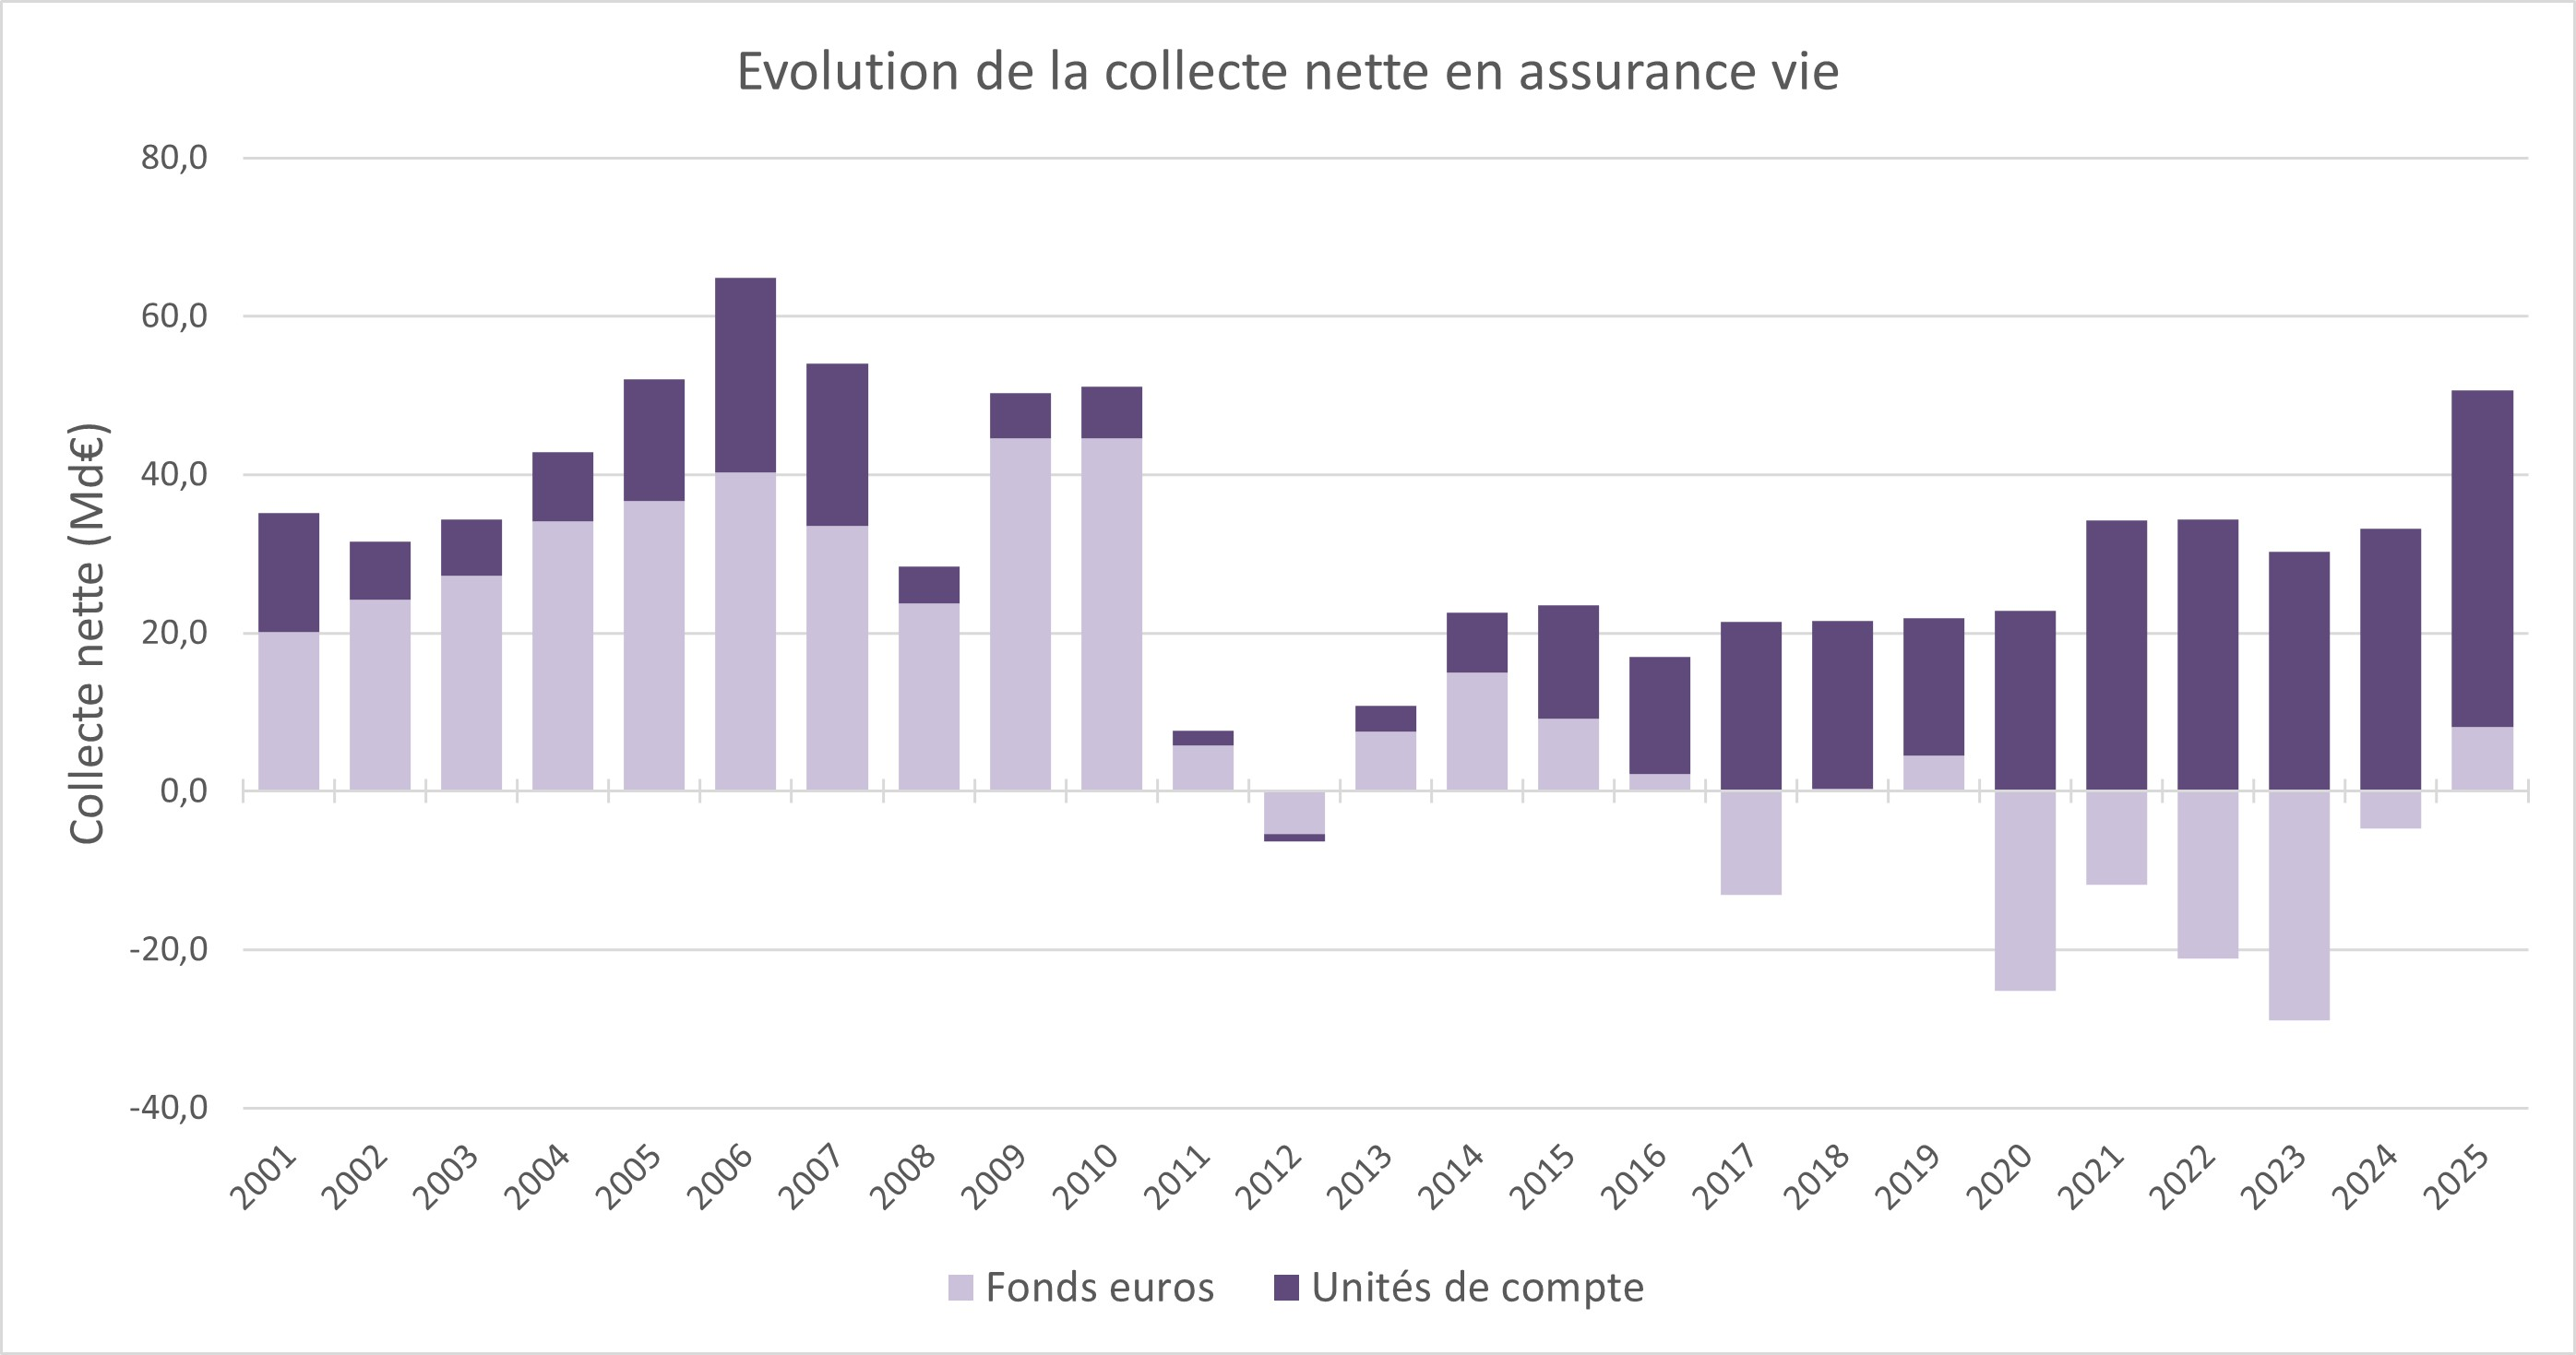
\includegraphics[scale=0.7]{images/evolution_collecte_nette.jpg}
    \caption{Evolution de la collecte nette en assurance vie en France entre 2000 et 2025}
    \label{fig:collecte_nette_assurance_vie_france}
\end{figure}

À partir de 2011, la collecte nette des fonds en euros s'est fortement tassée, traduisant l'érosion graduelle de leur attractivité dans un environnement durable de taux bas. Ce phénomène s'est ensuite accentué au début des années 2020 : entre 2020 et 2024, les fonds en euros ont enregistré une décollecte nette chaque année, atteignant un point particulièrement marqué en 2023 avec -28,9 milliards d'euros. 

À l'inverse, les unités de compte ont connu une dynamique nettement plus favorable. Leur collecte nette est restée positive chaque année depuis 2013 et a progressé de manière soutenue jusqu'à atteindre un niveau record de 42,5 milliards d'euros en 2025. Cette évolution montre que la croissance récente de l'assurance vie a été portée principalement par les supports en UC, alors même que les fonds en euros perdaient progressivement leur rôle de moteur commercial. Elle traduit ainsi un changement profond dans la structure des flux, désormais davantage orientés vers des supports où le risque financier est assumé, au moins en partie, par le souscripteur.

Cette transformation reflète clairement la stratégie d'adaptation mise en oeuvre par les assureurs. Confrontés à la compression des rendements obligataires et à la difficulté de maintenir l'attractivité des fonds en euros sans dégrader davantage leur marge financière, ils ont progressivement orienté leur offre vers des produits plus dynamiques, moins consommateurs de garanties et plus favorables du point de vue prudentiel. En parallèle, les épargnants ont été incités à diversifier davantage leur allocation, notamment au sein des contrats multisupports. La montée en puissance des unités de compte ne résulte donc pas seulement d'un changement de préférence des souscripteurs ; elle s'inscrit aussi dans une recomposition plus large du modèle économique de l'assurance vie, sous l'effet de l'environnement de taux.


\subsubsection{La stratégie sur l'actif}

Le quatrième axe a porté sur la gestion d'actifs et l'ALM. Dans le régime de taux bas, les assureurs ont dû arbitrer entre prudence et recherche de rendement. En réponse à cet environnement, de nombreux assureurs vie ont accru leur exposition à des actifs plus rémunérateurs mais aussi plus illiquides ou plus complexes, notamment les actifs alternatifs, l'immobilier, les prêts et certaines formes de dette privée ; à l'échelle européenne, ces actifs alternatifs représentaient 16 \% des investissements des assureurs à la fin de 2023. Cette stratégie de « search for yield » vise à reconstituer du rendement d'actif, mais elle s'accompagne de nouveaux risques : liquidité moindre, valorisations plus incertaines, dépendance à des primes d'illiquidité et plus grande complexité de gestion.

En France, cette adaptation de l'actif s'est accompagnée d'une gestion plus fine du risque de taux et de liquidité. La Banque de France souligne que les assureurs français recourent relativement peu aux swaps de taux par rapport à d'autres investisseurs institutionnels et privilégient davantage des couvertures de taux via options, notamment des caps, afin de se protéger contre une remontée des taux sans s'exposer à des appels de marge potentiellement déstabilisants. Ce point est important : compte tenu du caractère rachetable à tout moment des contrats d'assurance vie, la stratégie des assureurs ne consiste pas seulement à optimiser le rendement de l'actif, mais aussi à préserver la liquidité et à éviter qu'un choc de taux ne se transforme en choc de rachats.

Le cadre prudentiel a renforcé cette transformation stratégique. Sous Solvabilité II, la baisse des courbes sans risque accroît la valeur des provisions techniques et tend à réduire les ratios de solvabilité, surtout pour les assureurs vie. L'EIOPA observe précisément que la baisse des taux s'est traduite par une hausse significative de la valeur des engagements qui n'a pas été pleinement compensée par celle des actifs, d'où une pression sur les ratios de solvabilité. Le problème des taux bas n'est donc pas seulement un problème de rendement comptable ; il devient un enjeu de capital réglementaire et de résilience du bilan. C'est ce qui explique que les assureurs aient dû piloter simultanément la politique de participation aux bénéfices, la politique produit, l'allocation d'actifs et parfois même leur structure de financement.

\subsection{Les effets de la remontée des taux}

La remontée des taux amorcée à partir de 2022 a ouvert une nouvelle phase, plus favorable sur certains aspects mais non dénuée de risques. D'un côté, elle améliore progressivement la rentabilité future de l'actif, car les obligations arrivant à échéance peuvent être réinvesties à des rendements plus élevés. La Banque de France indique ainsi que le taux moyen de rendement de l'actif des assureurs vie est remonté à 2,5 \% en 2024, contre 2,2 \% en 2023 et 2,0 \% en 2022, mettant fin à la baisse quasi continue observée pendant la période de taux bas. D'un autre côté, cette remontée accroît la concurrence des placements bancaires liquides et peut alimenter un risque de rachats, surtout si la rémunération des fonds euros tarde à s'ajuster. Les autorités soulignent d'ailleurs que la hausse des taux depuis 2022 a conduit à une augmentation des rachats.

Les assureurs ont donc dû gérer une transition délicate : faire remonter suffisamment vite les rendements servis pour rester compétitifs, sans pour autant déstabiliser leur compte de résultat ni épuiser trop rapidement leurs réserves. En 2024, le maintien de taux de revalorisation attractifs, rendu possible par la hausse du rendement de l'actif et la mobilisation de la PPB, a permis une collecte nette très élevée sur le marché français. Mais cette amélioration ne remet pas en cause la transformation stratégique engagée depuis 2008 : la décennie de taux bas a durablement poussé les assureurs à réduire les garanties, à développer les UC, à affiner leur ALM, à diversifier davantage leurs placements et à inscrire la gestion du risque de taux au centre du pilotage du modèle d'affaires.

En définitive, depuis la crise de 2008, les taux directeurs ont agi comme un facteur structurant de la stratégie des assureurs vie. Dans la phase de taux bas, ils ont comprimé les marges, fragilisé les modèles fondés sur les garanties en capital et accéléré le basculement vers des produits moins consommateurs de capital et moins risqués pour l'assureur. Dans la phase de remontée récente, ils ont redonné des marges de manœuvre sur le rendement d'actif, tout en révélant un nouveau risque de concurrence et de rachats. L'effet stratégique des taux sur l'assurance vie ne peut donc pas être lu comme un simple choc conjoncturel ; il correspond à une reconfiguration durable du secteur, de ses produits et de ses équilibres prudentiels.





%%%%%%%%%%%%%%%%%%%%%%%%%%%%%%%
% Le contexte géopolitique actuel et son implication sur l'incertitude des taux
%%%%%%%%%%%%%%%%%%%%%%%%%%%%%%%
\section{Le contexte géopolitique actuel et son implication sur l'incertitude des taux}

Depuis 2020, l'environnement macroéconomique mondial est marqué par une succession de chocs exogènes qui ont profondément modifié le régime de taux d'intérêt. La pandémie de Covid-19 a d'abord provoqué un choc d'offre et de demande, conduisant les banques centrales à maintenir des politiques monétaires très accommodantes afin de soutenir l'activité économique. Par la suite, la reprise rapide de l'économie mondiale, les tensions sur les chaînes d'approvisionnement, puis la guerre en Ukraine ont entraîné une forte hausse des prix de l'énergie, des matières premières et des biens importés. Ces tensions ont alimenté une inflation durablement supérieure à la cible de 2 \% de la Banque centrale européenne, obligeant cette dernière à relever rapidement ses taux directeurs entre 2022 et 2023.

À ces facteurs s'ajoutent aujourd'hui d'autres sources d'incertitude géopolitique. Les tensions persistantes au Moyen-Orient, les rivalités commerciales entre grandes puissances, les risques de fragmentation des échanges internationaux et l'augmentation des dépenses militaires en Europe contribuent à rendre l'environnement économique plus instable. Ces éléments affectent les prix de l'énergie, les coûts de transport, les anticipations d'inflation et la confiance des agents économiques. Ainsi, même lorsque l'inflation ralentit, comme cela a été observé à partir de 2024, les banques centrales doivent rester prudentes dans leur trajectoire de baisse des taux. La BCE indique ainsi que la désinflation était en bonne voie début 2025, tout en réduisant progressivement le caractère restrictif de sa politique monétaire à partir de la mi-2024.

Le lien entre géopolitique et taux directeurs passe donc principalement par l'inflation et les anticipations d'inflation. Un choc géopolitique peut provoquer une hausse du prix du pétrole ou du gaz, une désorganisation des flux commerciaux ou une augmentation des coûts de production. Ces hausses de coûts se transmettent ensuite aux prix à la consommation. Si l'inflation observée ou anticipée s'éloigne de la cible de la banque centrale, celle-ci peut être conduite à maintenir des taux élevés plus longtemps, voire à les relever de nouveau. À l'inverse, si les tensions se résorbent et que l'inflation converge durablement vers l'objectif, la banque centrale peut assouplir sa politique monétaire. L'incertitude géopolitique se traduit donc par une incertitude sur la trajectoire future des taux courts.

Cette incertitude sur les taux directeurs se transmet ensuite à l'ensemble de la courbe des taux. Les taux courts sont directement influencés par les décisions de politique monétaire, tandis que les taux longs intègrent les anticipations de taux futurs, les anticipations d'inflation, la prime de terme et la perception du risque souverain. En période d'incertitude élevée, les investisseurs peuvent exiger une rémunération plus importante pour détenir des obligations longues, ce qui exerce une pression à la hausse sur les rendements obligataires. Les variations de taux ne sont donc pas seulement une conséquence mécanique des décisions de la BCE : elles reflètent également les anticipations des marchés concernant la croissance, l'inflation, la stabilité budgétaire et les risques internationaux.

Pour les assureurs-vie, cette dynamique est centrale en raison du poids important des obligations dans l'actif général, notamment au sein des fonds en euros. Lorsque les taux augmentent, la valeur de marché des obligations déjà détenues diminue. En effet, une obligation émise dans le passé avec un coupon faible devient moins attractive lorsque de nouvelles obligations offrent des rendements plus élevés. Cette baisse de valeur se traduit par des moins-values latentes dans le portefeuille obligataire. À l'inverse, lorsque les taux baissent, la valeur des obligations anciennes augmente, ce qui peut générer des plus-values latentes.

La remontée rapide des taux a donc eu un double effet pour les assureurs. À court terme, elle a pesé sur la valeur de marché des portefeuilles obligataires, en faisant apparaître des moins-values latentes importantes. Ce phénomène peut réduire la flexibilité financière de l'assureur, limiter sa capacité à réaliser des actifs sans pertes et fragiliser la gestion actif-passif en cas de rachats importants. À moyen terme, en revanche, la hausse des taux permet de réinvestir les flux obligataires arrivant à échéance dans des titres offrant des rendements plus élevés. Cela améliore progressivement le rendement courant du portefeuille et redonne de l'attractivité aux fonds en euros.

L'enjeu pour les assureurs-vie est donc de gérer une phase de transition. Les anciens portefeuilles, constitués pendant la longue période de taux bas, contiennent encore de nombreux titres faiblement rémunérés. Les nouveaux investissements, eux, bénéficient de conditions de rendement plus favorables. La vitesse d'amélioration du rendement moyen dépend alors de la duration du portefeuille, du rythme de renouvellement des actifs, du niveau des rachats et de la stratégie de réallocation mise en œuvre par l'assureur. 

Cette situation influence également le passif des assureurs-vie. Lorsque les taux de marché augmentent, les épargnants comparent davantage le rendement des fonds en euros avec celui d'autres produits de taux, comme les livrets réglementés, les comptes à terme ou les obligations détenues en direct. Si le rendement servi sur les contrats d'assurance-vie ne s'ajuste pas suffisamment vite, le risque de rachats augmente. Les assureurs doivent alors arbitrer entre la préservation de leurs marges, l'utilisation éventuelle de la provision pour participation aux bénéfices et le maintien de l'attractivité commerciale des contrats. Dans un contexte de remontée des taux, la concurrence entre produits d'épargne devient donc plus forte.

L'incertitude géopolitique renforce ainsi l'incertitude financière des assureurs-vie. Un nouveau choc inflationniste pourrait conduire à un maintien prolongé des taux élevés, ce qui prolongerait les tensions sur les portefeuilles obligataires existants. À l'inverse, une baisse rapide de l'inflation pourrait accélérer l'assouplissement monétaire, soutenir la valeur de marché des obligations et améliorer les plus-values latentes. Toutefois, une baisse trop rapide des taux réduirait aussi le rendement des futurs réinvestissements. L'assureur-vie est donc exposé non seulement au niveau des taux, mais aussi à leur volatilité et à l'incertitude entourant leur trajectoire.

Dans ce contexte, la gestion actif-passif devient un outil déterminant. Les assureurs doivent piloter la duration de leurs actifs, anticiper les comportements de rachat, mesurer l'impact de différents scénarios de taux et maintenir un équilibre entre rendement, liquidité et solvabilité. Les travaux de l'EIOPA soulignent d'ailleurs que les assureurs européens évoluent dans un environnement marqué par une croissance fragile, des incertitudes élevées et des risques géopolitiques persistants.

Ainsi, le contexte géopolitique actuel constitue un facteur majeur d'incertitude pour l'assurance-vie. Il agit d'abord sur les prix de l'énergie, les chaînes de valeur et les anticipations d'inflation, puis sur les décisions de politique monétaire et la courbe des taux. Ces mouvements affectent directement la valorisation des portefeuilles obligataires, les plus ou moins-values latentes, les conditions de réinvestissement, le comportement des assurés et la solvabilité des organismes. L'incertitude des taux directeurs ne peut donc pas être analysée isolément : elle s'inscrit dans un environnement macroéconomique et géopolitique plus large, qui conditionne à la fois l'actif et le passif des assureurs-vie.
%%%%%%%%%%%%%%%%%%%%%%%%%%%%%%
% Les contraintes réglementaires
%%%%%%%%%%%%%%%%%%%%%%%%%%%%%%
\section{Les contraintes réglementaires}
A définir si vraiment utile
\subsection{Le cadre réglementaire de Solvabilité II}
\subsection{Le cadre réglementaire de IFRS 17}